\documentclass[a4paper,10pt]{article}

%A Few Useful Packages
\usepackage{marvosym}
\usepackage{fontspec} 					%for loading fonts
\usepackage{xunicode,xltxtra,url,parskip} 	%other packages for formatting
\RequirePackage{color,graphicx}
\usepackage[usenames,dvipsnames]{xcolor}
%\usepackage[big]{layaureo} 				%better formatting of the A4 page
% an alternative to Layaureo can be ** \usepackage{fullpage} **
\usepackage[empty]{fullpage}
\usepackage{supertabular} 				%for Grades
\usepackage{titlesec}					%custom \section
\usepackage{tabu}
\usepackage{multirow}
\usepackage{hyperref}


%Setup hyperref package, and colours for links
\usepackage{hyperref}
\definecolor{linkcolour}{rgb}{0,0.2,0.6}
\hypersetup{colorlinks,breaklinks,urlcolor=linkcolour, linkcolor=linkcolour}

%FONTS
\defaultfontfeatures{Mapping=tex-text}
%\setmainfont[SmallCapsFont = Fontin SmallCaps]{Fontin}
%%% modified for Karol Kozioł for ShareLaTeX use
\setmainfont[
SmallCapsFont = Fontin-SmallCaps.otf,
BoldFont = Fontin-Bold.otf,
ItalicFont = Fontin-Italic.otf
]
{Fontin.otf}
%%%

%CV Sections inspired by: 
%http://stefano.italians.nl/archives/26
\titleformat{\section}{\Large\scshape\raggedright}{}{0em}{}[\titlerule]
\titlespacing{\section}{0pt}{2pt}{2pt}
%Tweak a bit the top margin
   \addtolength{\voffset}{-0.7cm}
%\vsize=15cm
%\setlength{\footskip}{.96cm}
%\def\makefootline{\baselineskip24pt\lineskiplimit0pt\line{\the\footline}}
%\vsize 180mm
%\addtolength{\vsize}{-50cm}
%Italian hyphenation for the word: ''corporations''
\hyphenation{im-pre-se}

%-------------WATERMARK TEST [**not part of a CV**]---------------
\usepackage[absolute]{textpos}

\setlength{\TPHorizModule}{30mm}
\setlength{\TPVertModule}{\TPHorizModule}
\textblockorigin{2mm}{0.80\paperheight}
\setlength{\parindent}{0pt}
%\setlength{\topsep}{5pt}%

%--------------------BEGIN DOCUMENT----------------------
\begin{document}

\pagestyle{empty} % non-numbered pages

\font\fb=''[cmr10]'' %for use with \LaTeX command

%--------------------TITLE-------------


%\begin{figure}[!t]
%\begin{flushleft}
%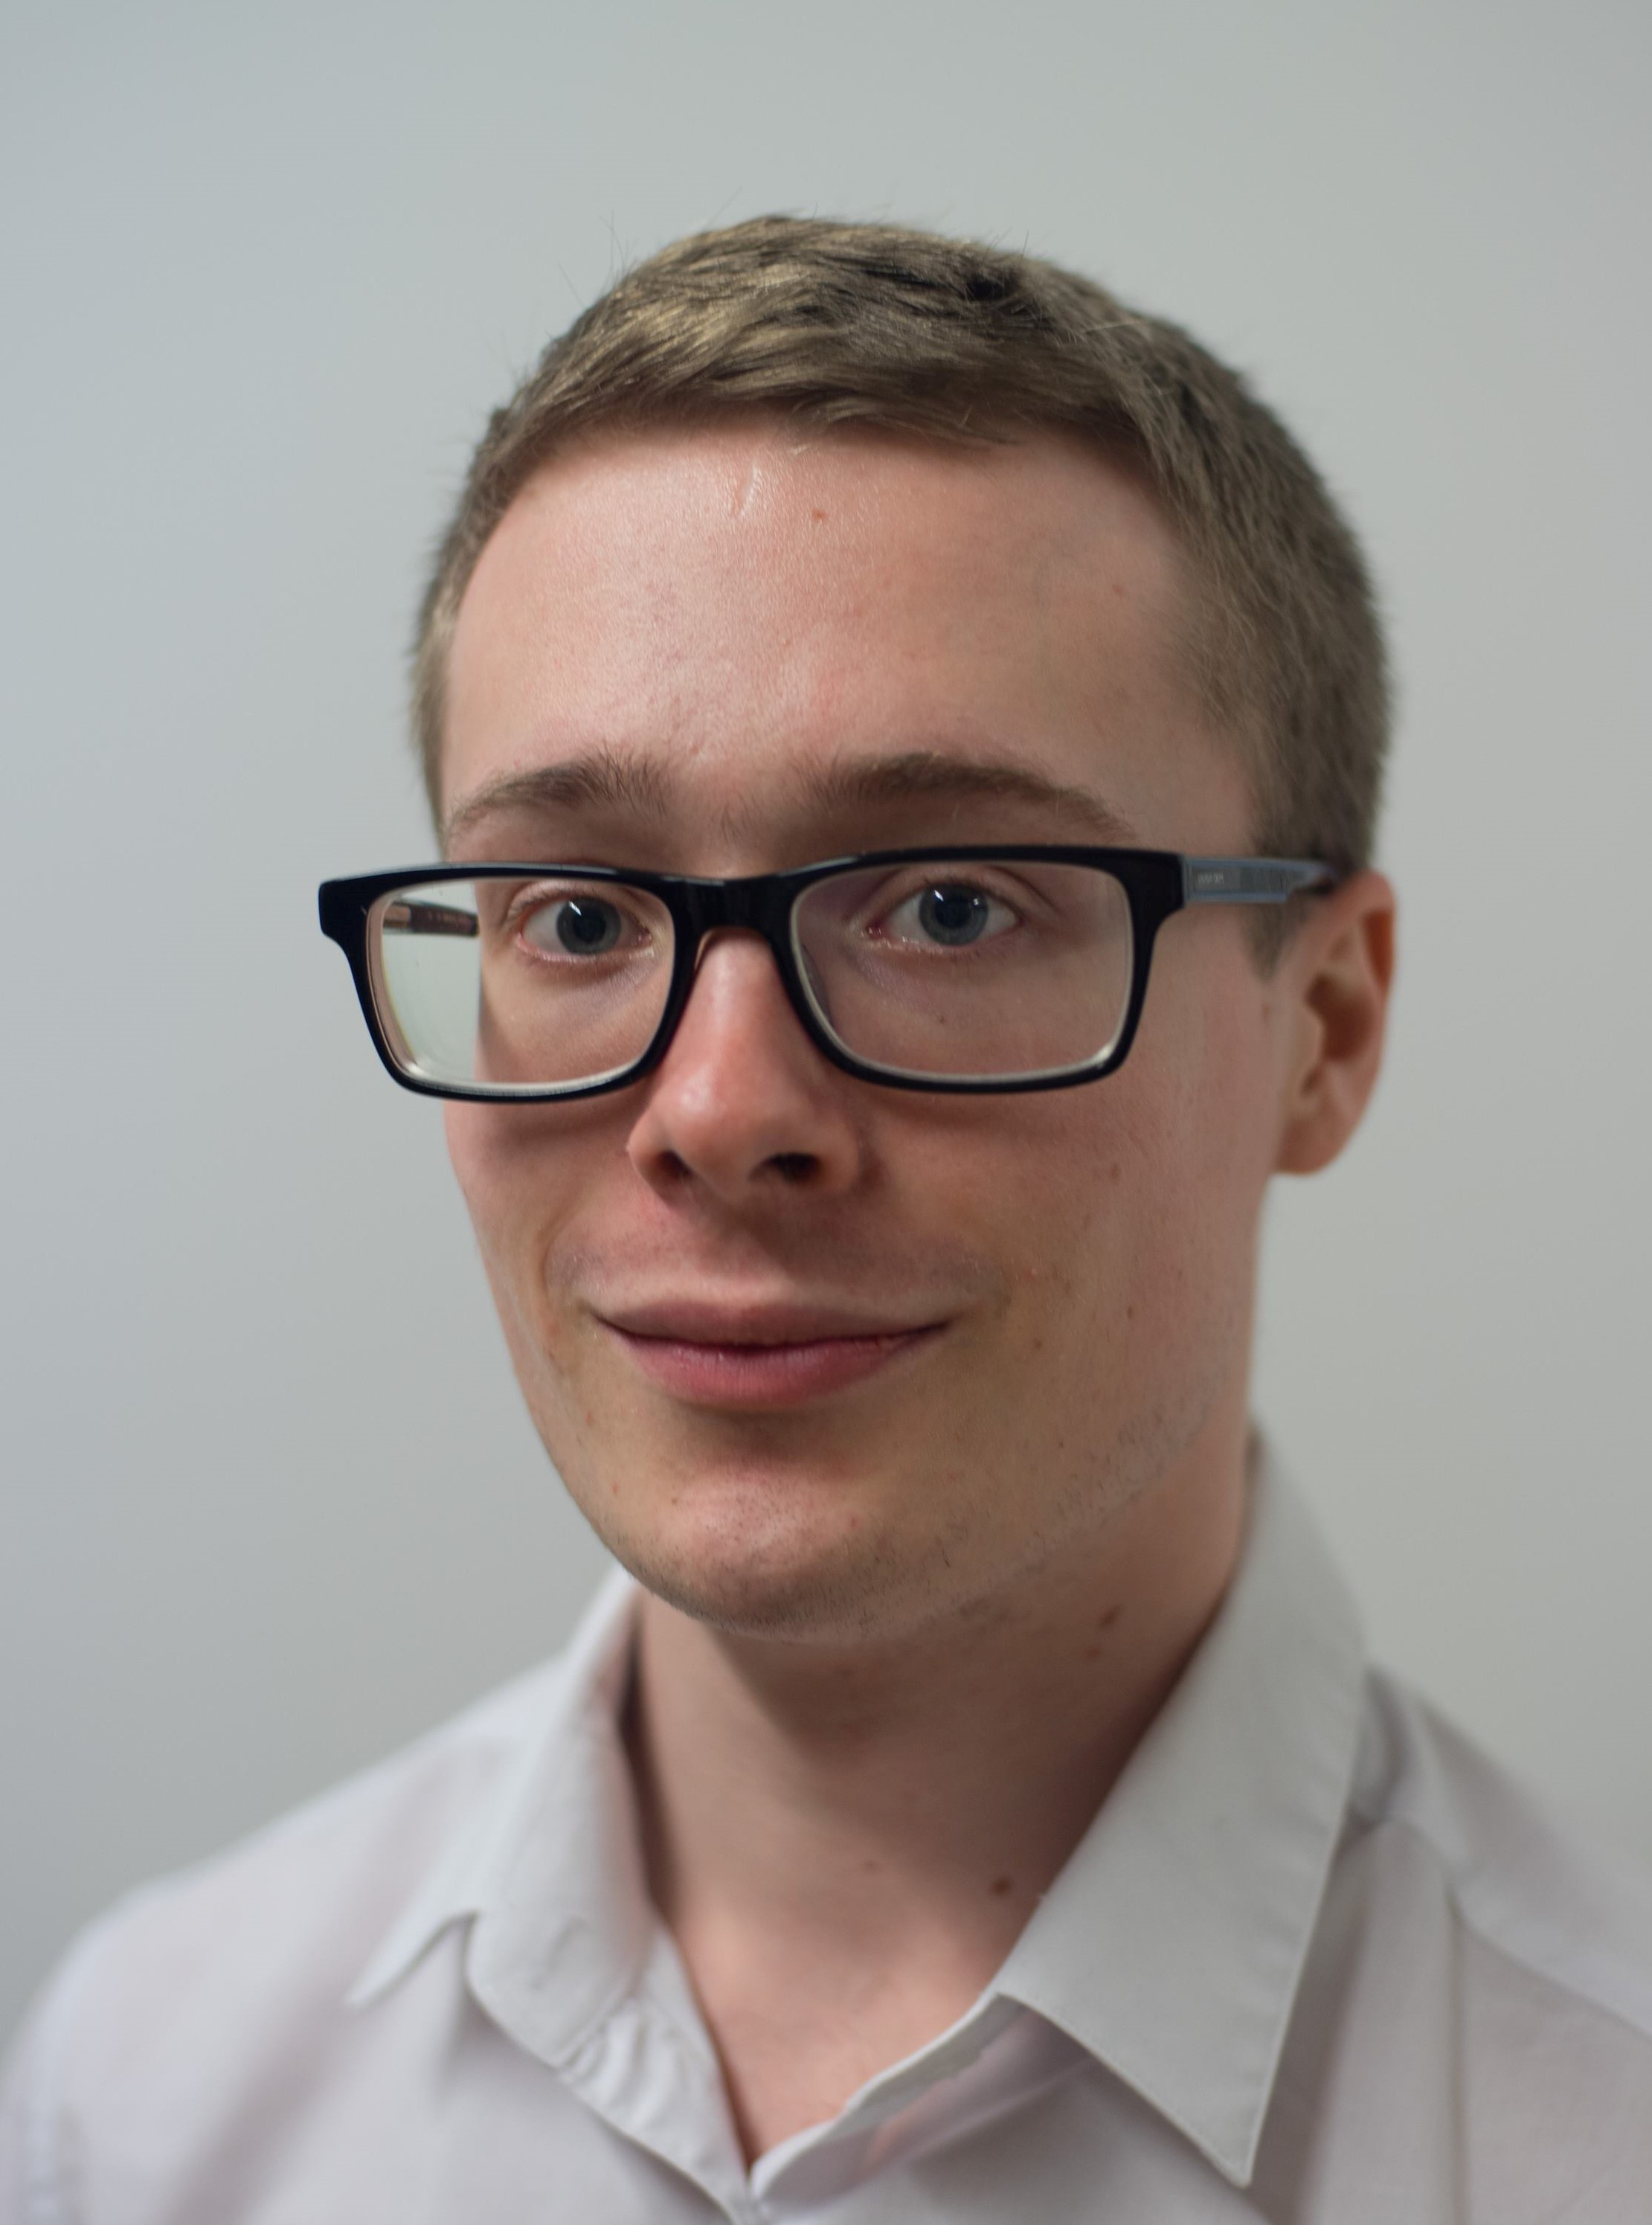
\includegraphics[width=1.5in]{pic}
%\end{flushleft}
%\end{figure}
  %\vspace{-5in}
  \begin{tabular}{ p{11.5cm}r }
   %& %\multirow{1}{2in}%{
   %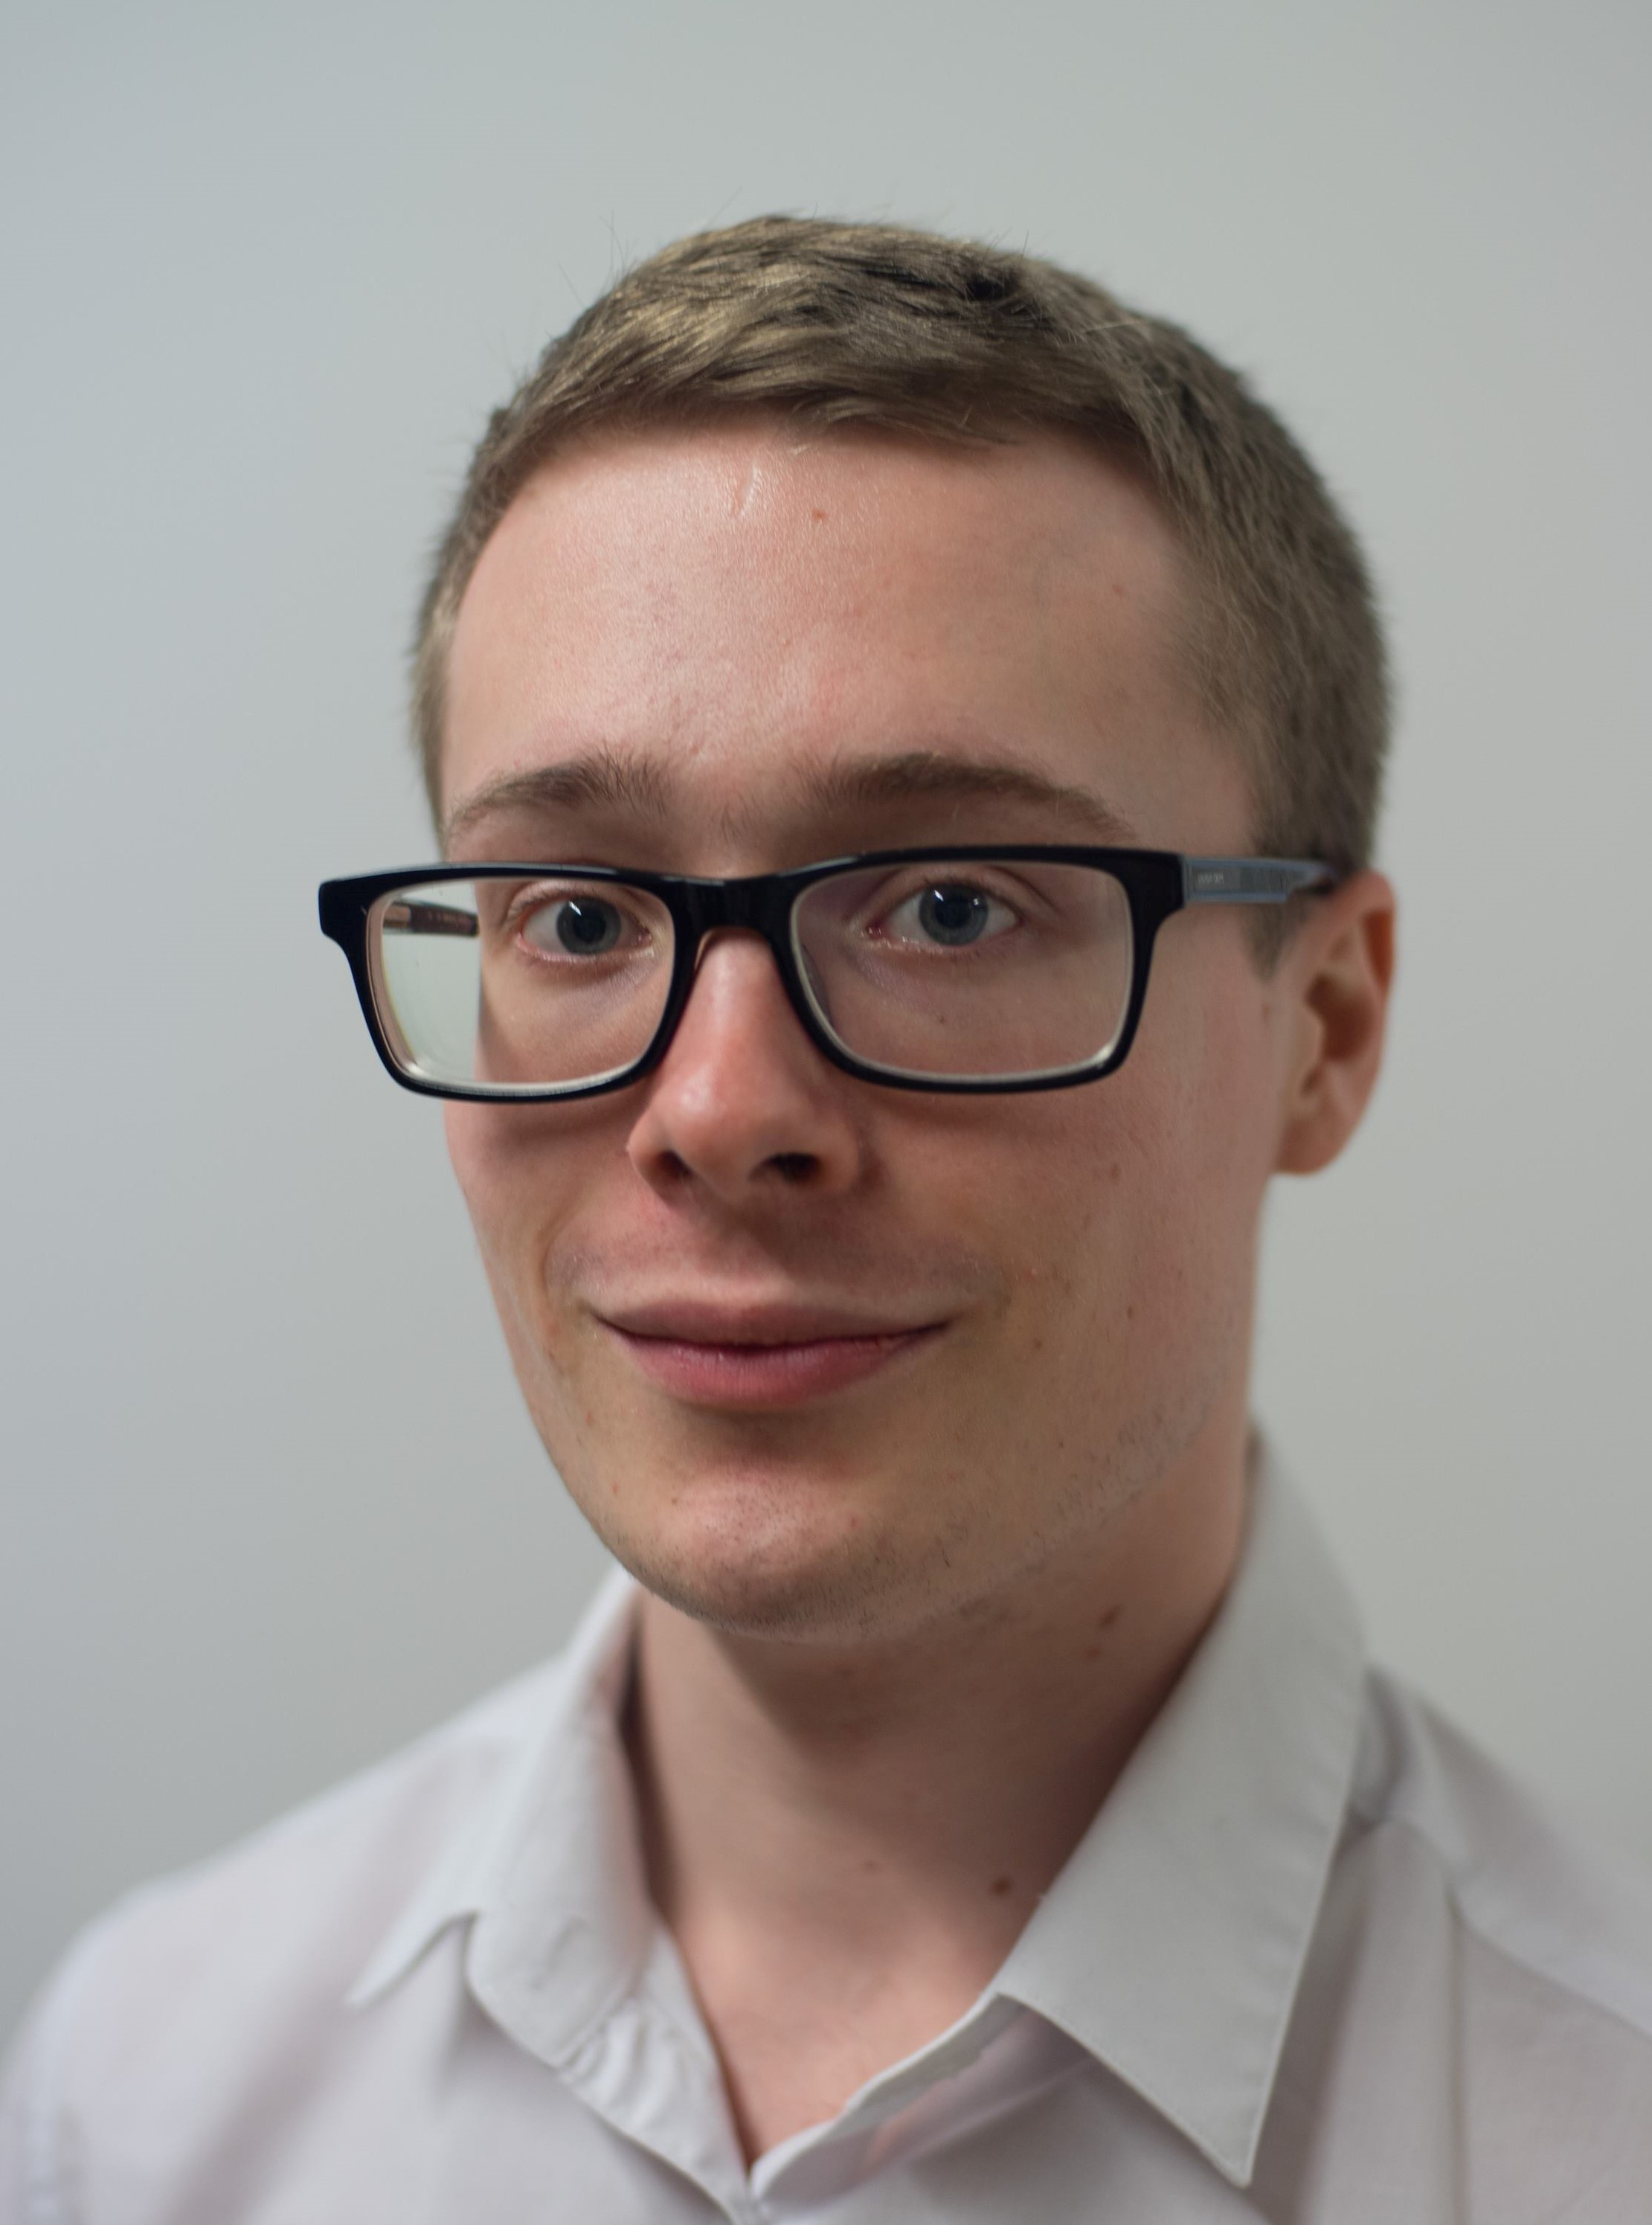
\includegraphics[width=1.5in]{pic}\\
   %} \\
   & \multirow{2}{*}{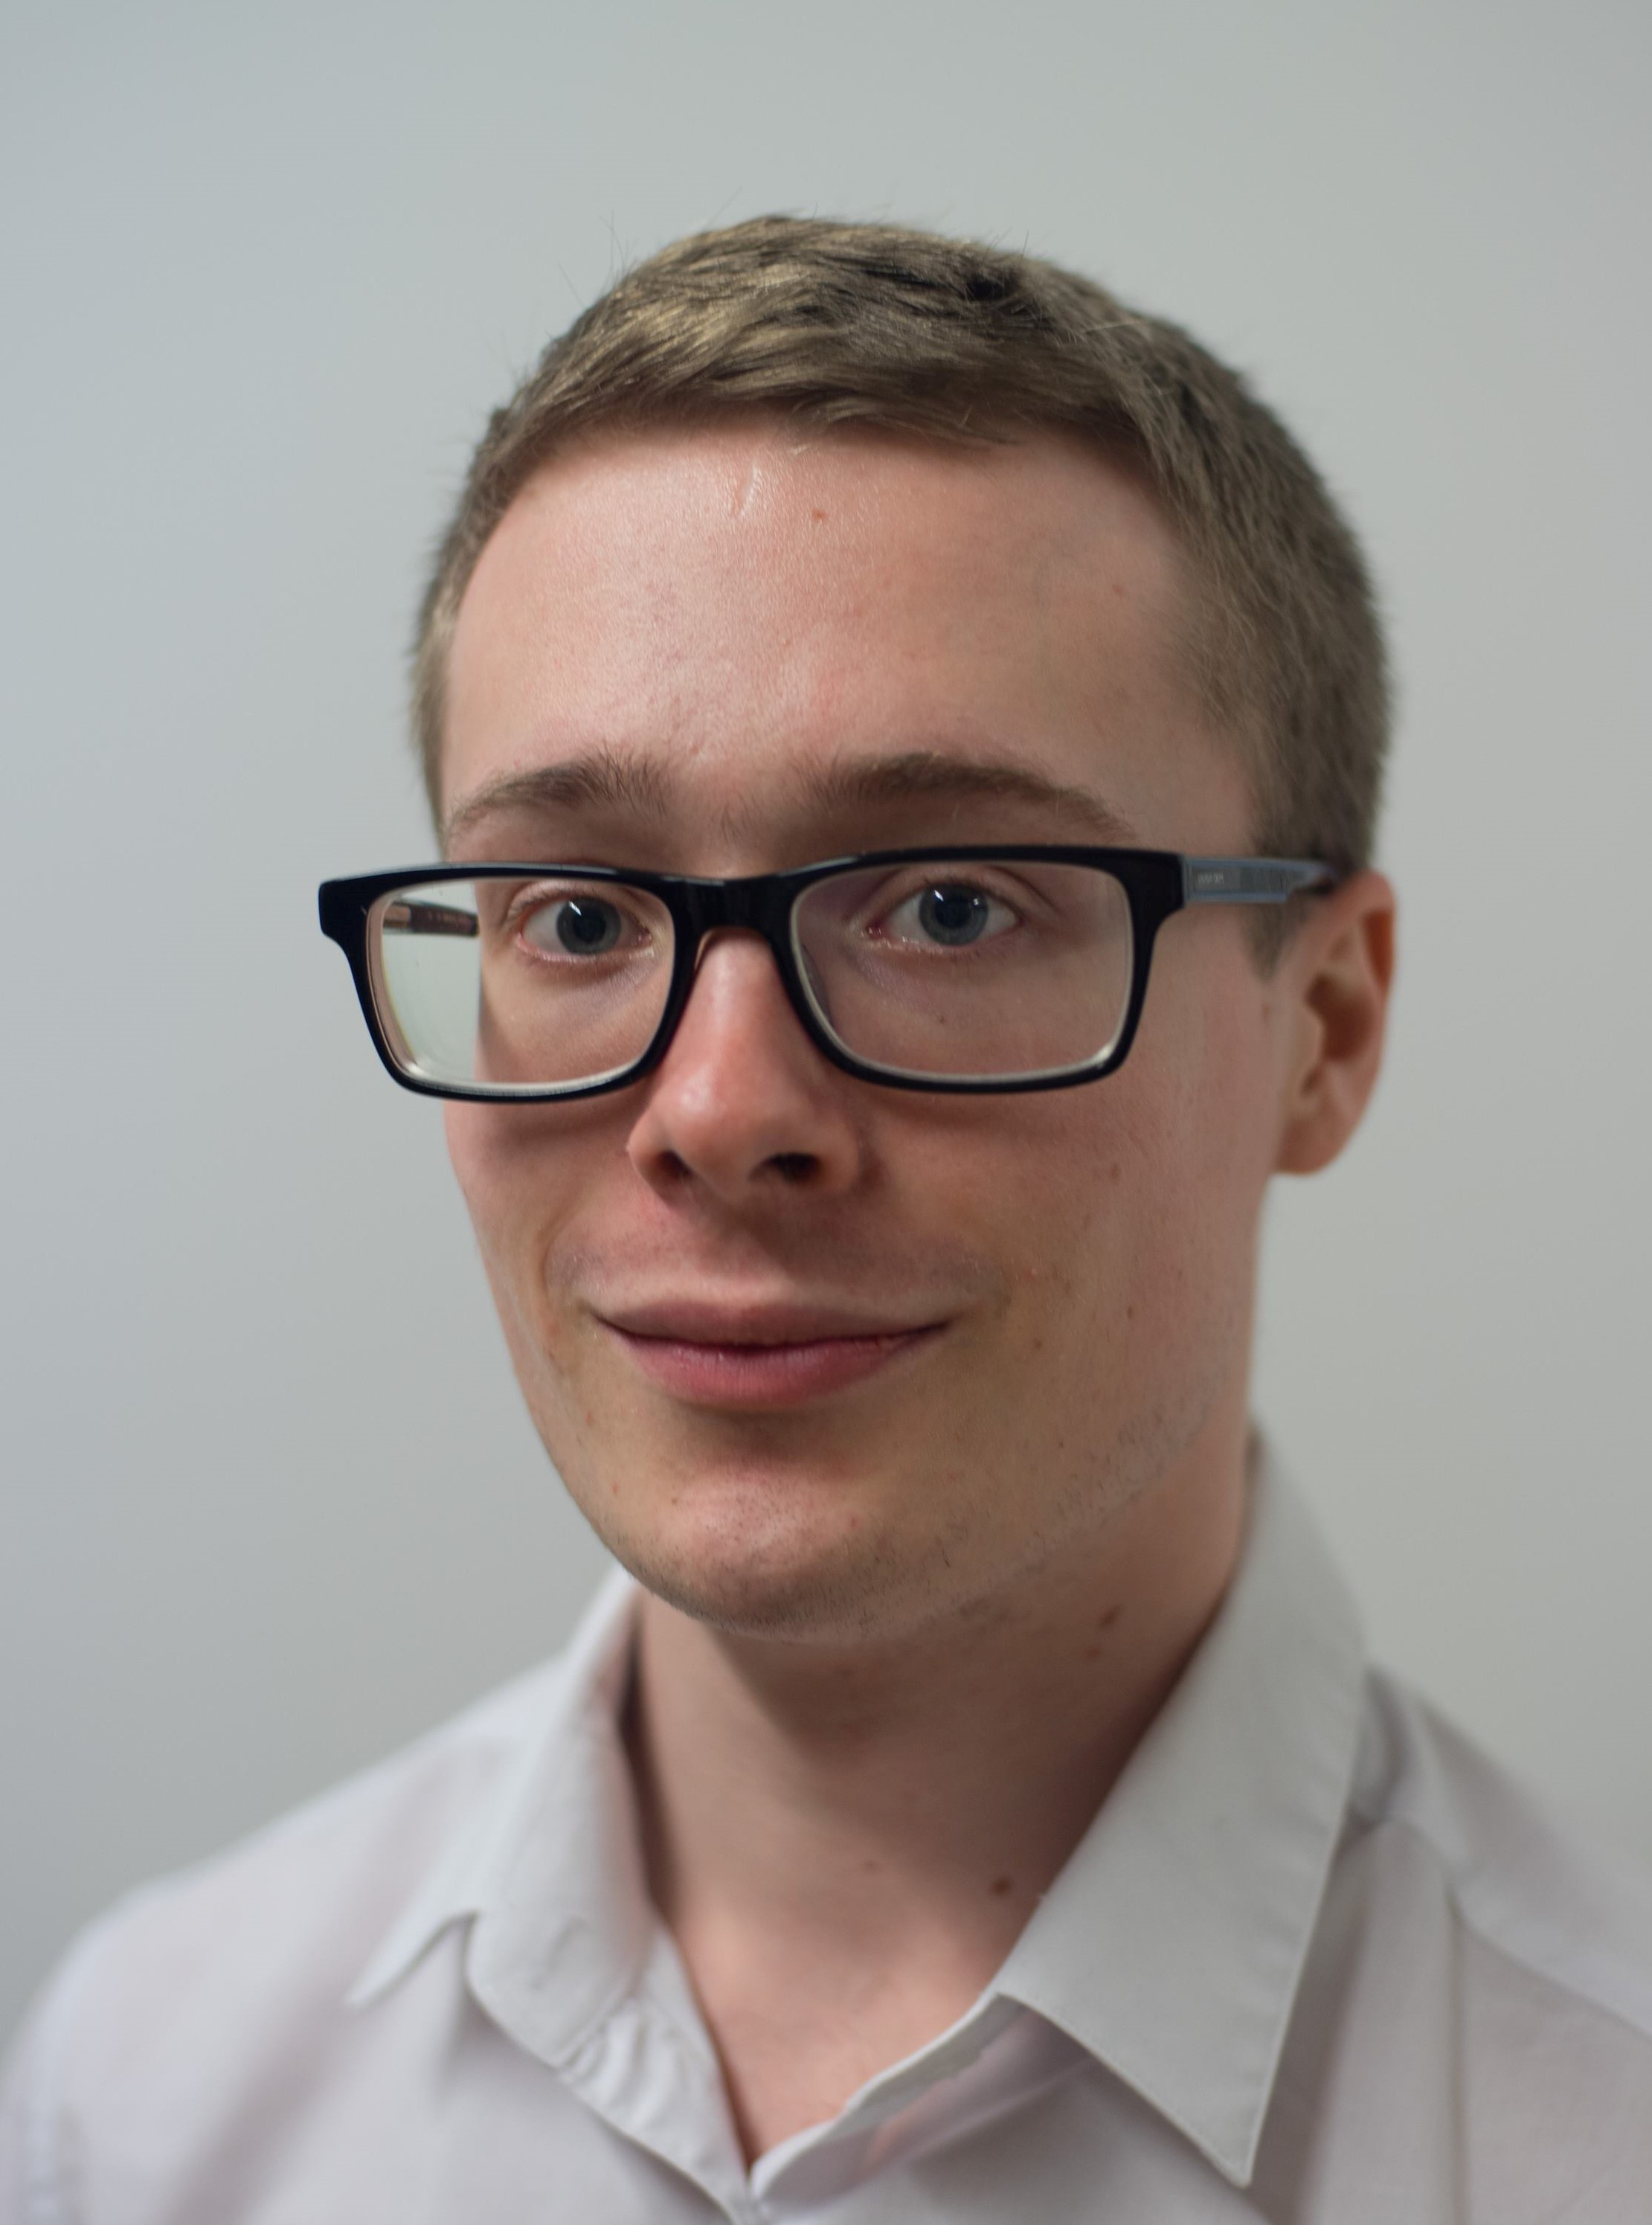
\includegraphics[width=1.3in]{pic}}\\
   \\
   \scshape{\Huge{Charles Nourry}} & \\
   \\
   \textsc{Age:} 21 ans &\\
    \textsc{Adresse:} 1 rue de la ferme &\\
    \textsc{Ville:} 78150 - Le Chesnay&\\
    \textsc{Téléphone:} 06 21 09 85 62&\\
    \textsc{email:} \href{mailto:nourry\_charles@outlook.fr}{nourry\_charles@outlook.fr}& %\multirow{5}{2in}{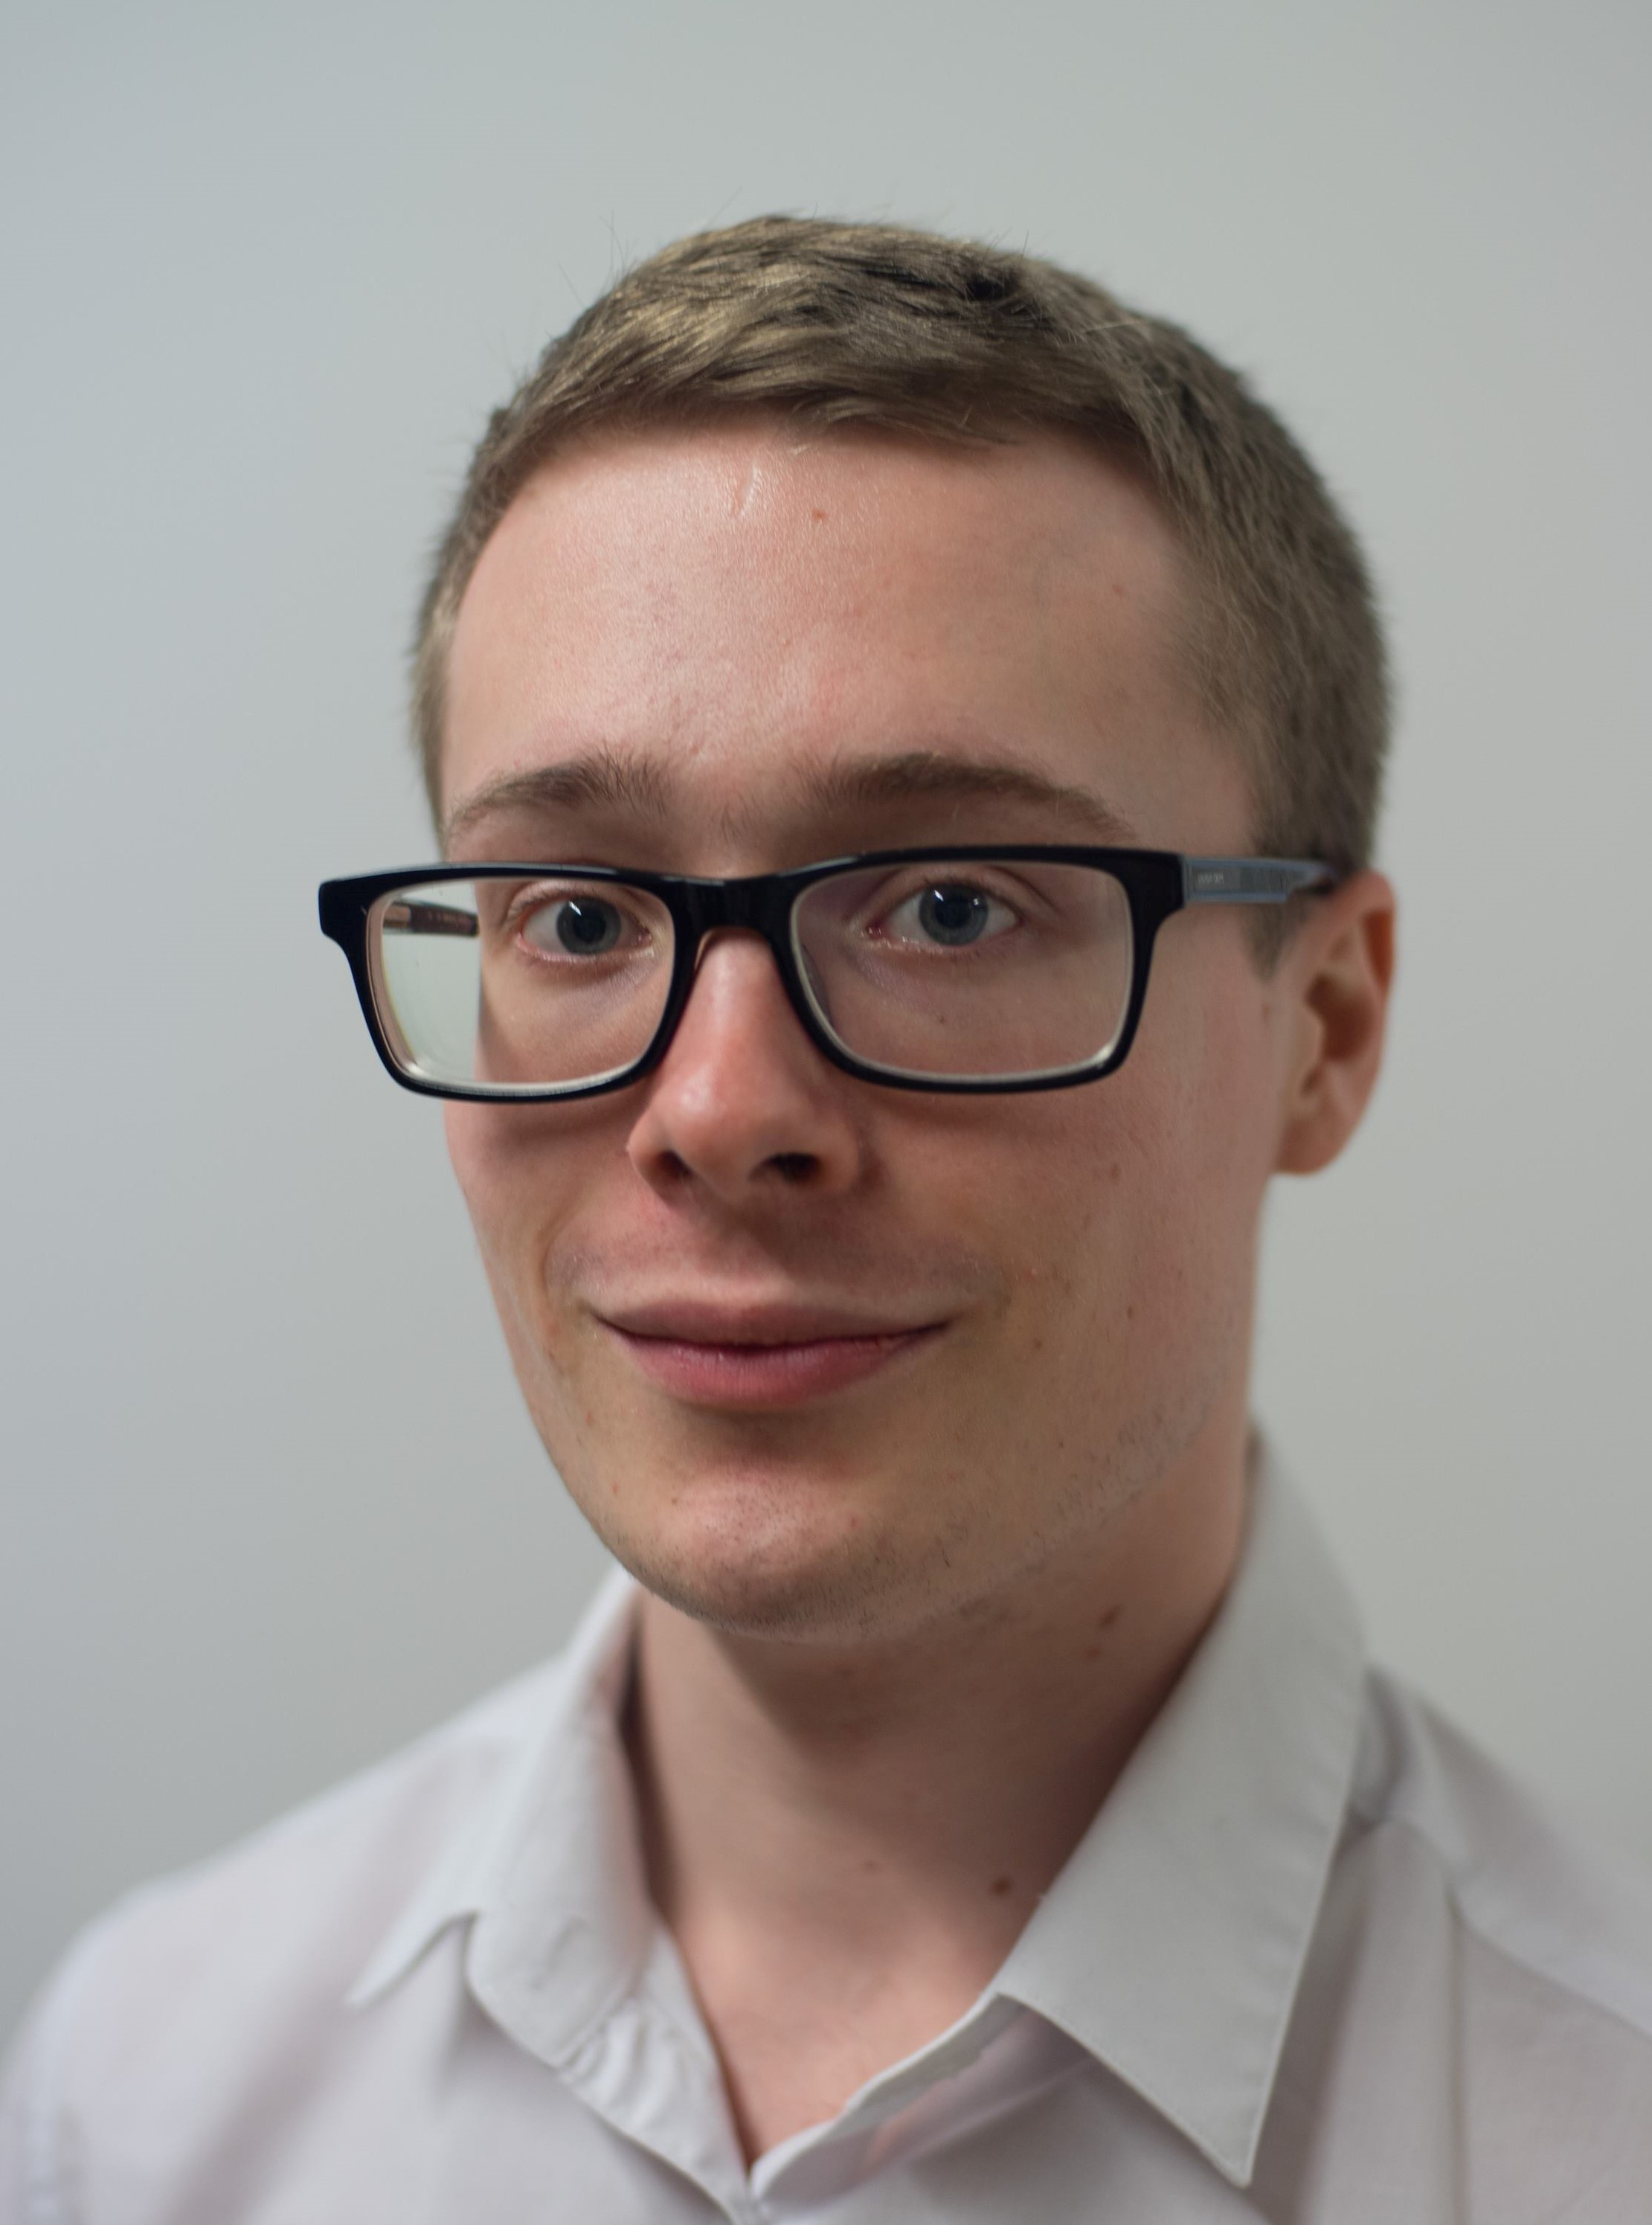
\includegraphics[width=1.5in]{pic}}
  \end{tabular}
  
  \vspace{0.3in}
  \centering{
  \Large{Candidature à l'offre de stage : Optimisation de l’insertion de contre mesure pour la sécurité des Circuits Intégrés}
}
%\par{%\centering{
%	\Large
%	Charles \textsc{Nourry}
	%}
%	\bigskip\par}
%\normalsize
%--------------------SECTIONS-----------------------------------
%Section: Personal Data
%\section{Personal Data}

%\begin{tabular}{ll}
 %   \textsc{Age:} & 20 \\
  %  \textsc{Address:}   & 1 rue de la ferme \\
%    \textsc{Ville:} 	& 78150 - Le Chesnay\\
 %   \textsc{Phone:}     & 06 21 09 85 62\\
  %  \textsc{email:}     & $\href{mailto:nourry_charles@outlook.fr}{nourry_charles@outlook.fr}$
%\end{tabular}

%Section: Work Experience at the top
\section{Formation}
\begin{tabular}{r|p{12.5cm}}
 \textsc{2017-2019} & Master 2 Modélisation, Optimisation, Décision et Organisation \\&\emph{\small{Cohabilité par Université Paris-Dauphine et Mines ParisTech}}\\\multicolumn{2}{c}{} \\
 \textsc{2016-2017} & Licence Informatique des organisations - MIAGE et Décision \\&\emph{\small{Université Paris-Dauphine}}\\\multicolumn{2}{c}{} \\
 \textsc{2014-2016} & Diplôme d'Etablissement Mathématiques, Informatique et applications à l'Economie et à l'Entreprise (L1 \& L2) \\&\emph{\small{Université Paris-Dauphine}}\\\multicolumn{2}{c}{} \\
 \textsc{2014} & Baccalauréat Scientifique option Mathématiques \\&\emph{\small{Lycée Blanche de Castille, Le Chesnay}}\\
\end{tabular}
\titlespacing{\section}{0pt}{2pt}{2pt}
\section{Expériences personnelles}
\begin{tabular}{cl}	
 \textsc{Mai} 2018 & Stage de recherche au \textsc{LAMSADE} (Laboratoire d'Analyse et Modélisation de\\ \textsc{Août} 2018 & Systèmes pour l'Aide à la Décision) - Université Paris-Dauphine\\
  & \emph{"Analyse de débats en ligne"}\small{ | Etudes et modélisations de débats à l'aide de la théorie }\\& \small{de l'argumentation}\\&\\
 \textsc{Mai} 2017 & Stage de Licence au \textsc{Crédit Industriel et Commercial}\\
 \textsc{Août} 2017 & \emph{"Mise en place d'outils informatiques"}\small{ | Gestion de bases de données et élaborations d'applications}\\&\\
 2016-2018 & Projets universitaires : Gestion d'emplois du temps, Modélisation de problèmes de\\& gestion, Résolution de puzzles (\emph{infinityloop}), Réseaux de neurones, Intelligence \\&Artificielle pour résoudre des jeux(\emph{domineering, sudoku, dominos...})
\end{tabular}

\section{Compétences}
\begin{tabular}{ll}	
\textsc{Développement :} & Programmation orientée objet, Java, C, Python, R, Matlab, \LaTeX, VBA\\

\textsc{Logiciels/OS :} & Microsoft Windows, Linux, Word, Excel, PowerPoint, Access, Eclipse, JetBrains \\&(\emph{IntelliJ, CLion, PyCharm,...}), CPlex Studio, GitHub, Jupyter Notebook, RStudio, MySQL
\end{tabular}

%Section: Languages
\section{Langues}
\begin{flushleft}
\begin{tabular}{p{0.4cm}lll}
&\textsc{Français :}&Langue maternelle\\
&\textsc{Anglais :}&Courant (TOEIC 2018: 820/990)\\
&\textsc{Espagnol :}&Occasionnel
\end{tabular}
\end{flushleft}

\section{Centres d'intérêt}
\begin{flushleft}
Piano, Cinéma, Athlétisme
\end{flushleft}
%\XeTeXpdffile ''GMAT.pdf'' page 1 scaled 800

\end{document}
